\section{Random Matrix filtering}
\label{sec:rmt}

\subsection{Empirical eigenspectrum}

Random Matrix Theory supplies the spectral benchmark for distinguishing structured collective modes from sampling noise in the empirical correlation matrix \cite{laloux_1999_noise,plerou_2002_random}. The core historical matrix uses $N=58$ assets and $T=1527$ observations, giving $Q=T/N\approx26.33$. The Mar\v{c}enko--Pastur bounds are $\lambda_-=0.6482$ and $\lambda_+=1.4278$.

\begin{center}
\captionof{table}{RMT summary for the core historical universe.}
\label{tab:rmt_summary}
\resizebox{\linewidth}{!}{%
\begin{tabular}{rrrrrrrrrrr}
\toprule
$N$ & $T$ & $Q$ & $\lambda_-$ & $\lambda_+$ & $\lambda_1$ & $\lambda_2$ & $\lambda_3$ & $\lambda_4$ & $\lambda_5$ & Above $\lambda_+$ \\
\midrule
58 & 1527 & 26.33 & 0.6482 & 1.4278 & 21.6505 & 3.0957 & 1.7839 & 1.6543 & 1.4835 & 5 \\
\bottomrule
\end{tabular}}
\end{center}

Table~\ref{tab:rmt_summary} reports the numerical inputs for RMT filtering. With $N=58$ assets and $T=1527$ complete observations, the aspect ratio is $Q=26.33$, which implies a relatively narrow Mar\v{c}enko--Pastur noise band from $\lambda_-=0.6482$ to $\lambda_+=1.4278$. The first eigenvalue, $\lambda_1=21.6505$, is therefore not a marginal deviation from the random-matrix benchmark but a dominant collective component. The next four eigenvalues, $\lambda_2=3.0957$, $\lambda_3=1.7839$, $\lambda_4=1.6543$ and $\lambda_5=1.4835$, also exceed the upper random bound. There are 5 sample eigenvalues outside the band: these are the candidate collective modes, indicating one broad market mode and four additional modes that may be associated with group, sectoral or localized dependency structure.

Figure~\ref{fig:rmt_spectrum} shows the spectrum against the random benchmark. The largest eigenvalue lies far above the Mar\v{c}enko--Pastur upper bound. Four additional eigenvalues also exceed the upper edge, indicating a dominant market mode and a small number of group or sector modes.

\begin{center}
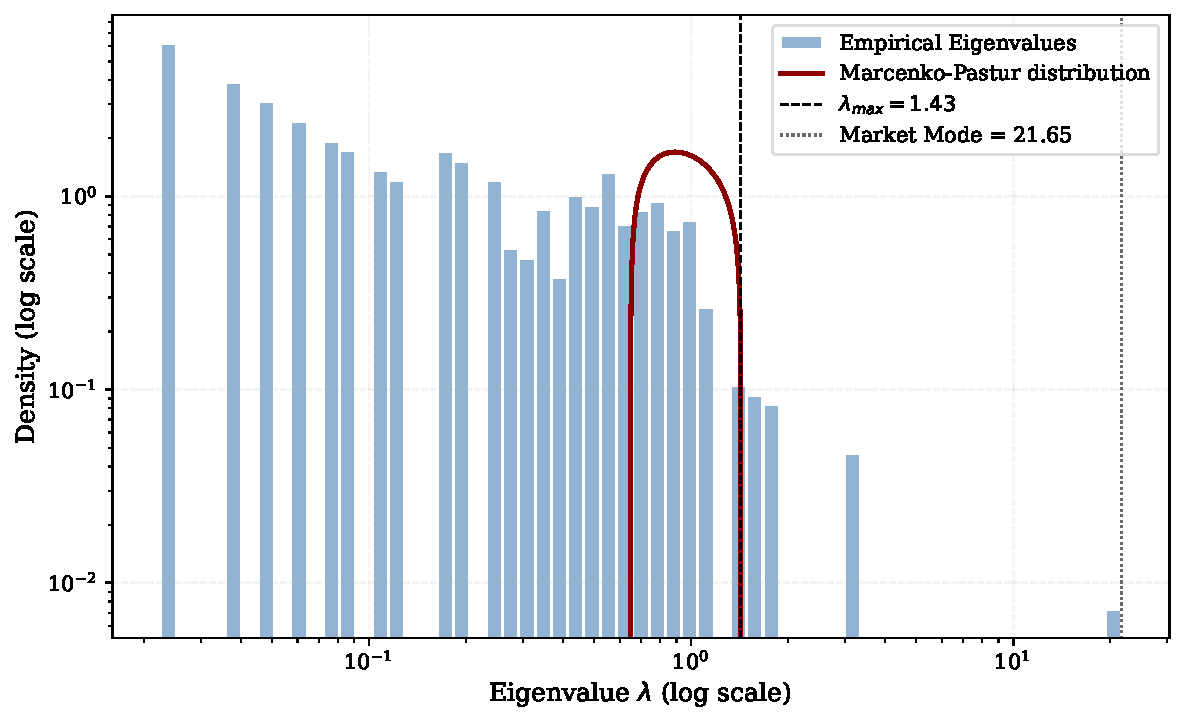
\includegraphics[width=0.88\linewidth]{images/figure_6_rmt_eigenvalue_spectrum.pdf}
\captionof{figure}{Empirical eigenvalue spectrum and Mar\v{c}enko--Pastur bounds. The largest eigenvalue is far outside the random band and captures the market-mode component.}
\label{fig:rmt_spectrum}
\end{center}


\subsection{Market Mode and significant eigenvalues}

The largest eigenvalue is 21.6505, corresponding to approximately 37.3\% of the total trace of the correlation matrix. Its eigenvector has broadly positive loadings, confirming its interpretation as a market mode. It captures broad co-movement and explains why the original correlation matrix has a strong positive common component. The next four eigenvalues are 3.0957, 1.7839, 1.6543 and 1.4835. These values are above $\lambda_+$ and act as candidates for group or sector structure.

The market mode is meaningful but visually dominant. If a network is built directly from the original matrix, many edges can reflect market-wide co-movement instead of local structure. We construct the group-mode matrix to ask what remains after the broad common component is removed.


\subsection{Matrix reconstruction}

The reconstruction step checks that the spectral decomposition and the filtered matrices are being computed accurately. If all eigenvalue--eigenvector modes are recombined, the original correlation matrix is recovered up to floating-point precision. Table~\ref{tab:rmt_reconstruction} reports this numerical check: the Frobenius reconstruction error is approximately $2.74\times10^{-14}$, and the maximum absolute reconstruction error is approximately $3.99\times10^{-15}$. The reported unit diagonal refers to the filtered matrix after the partial reconstruction has been rescaled for downstream correlation-based distances. This check reduces the possibility that subsequent network differences are driven by numerical reconstruction error rather than by the intended selection of market, group and noise-compatible modes.

\begin{center}
\captionof{table}{RMT reconstruction diagnostics.}
\label{tab:rmt_reconstruction}
\begin{tabular}{lr}
\toprule
Diagnostic & Value \\
\midrule
Frobenius reconstruction error & $2.74\times10^{-14}$ \\
Maximum absolute reconstruction error & $3.99\times10^{-15}$ \\
$C_{\mathrm{filtered}}$ diagonal min & 1.0000 \\
$C_{\mathrm{filtered}}$ diagonal max & 1.0000 \\
Eigenvalues above $\lambda_+$ & 5 \\
Market-mode trace share & 0.3733 \\
\bottomrule
\end{tabular}
\end{center}

Figure~\ref{fig:rmt_filtered_matrices} shows the resulting matrix components. The original-correlation panel is the complete empirical correlation matrix used throughout the paper. The market-mode matrix captures broad positive co-movement. The group-mode matrix displays weaker localized patterns after the market mode is removed. The noise component contains the random-band contribution, and the filtered matrix recombines the retained modes.

Empirically, the eigenvectors beyond the leading component show loading patterns suggesting localized or sector-related dependencies. This residual organization motivates the clustering and network sections: if localized dependency patterns remain after market-mode removal, MST and PMFG structures should differ when constructed from the group-mode matrix.

\begin{center}
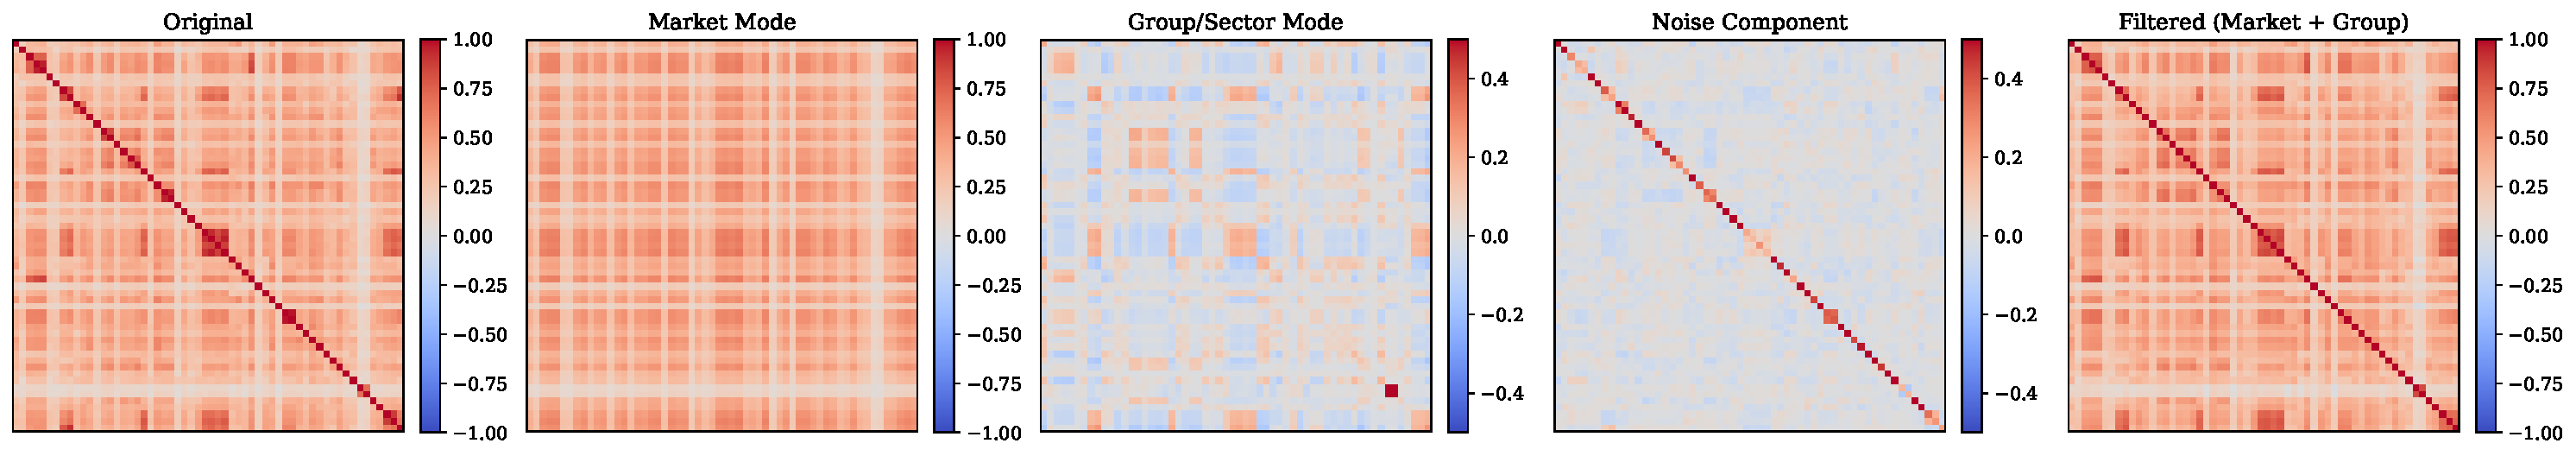
\includegraphics[width=\linewidth]{images/figure_8_rmt_filtered_matrices.pdf}
\captionof{figure}{Empirical and RMT-filtered matrix components. The original-correlation panel shows the complete 58-asset correlation matrix; the remaining panels separate it into market, group/sector, noise and filtered components.}
\label{fig:rmt_filtered_matrices}
\end{center}

\clearpage

\begin{center}
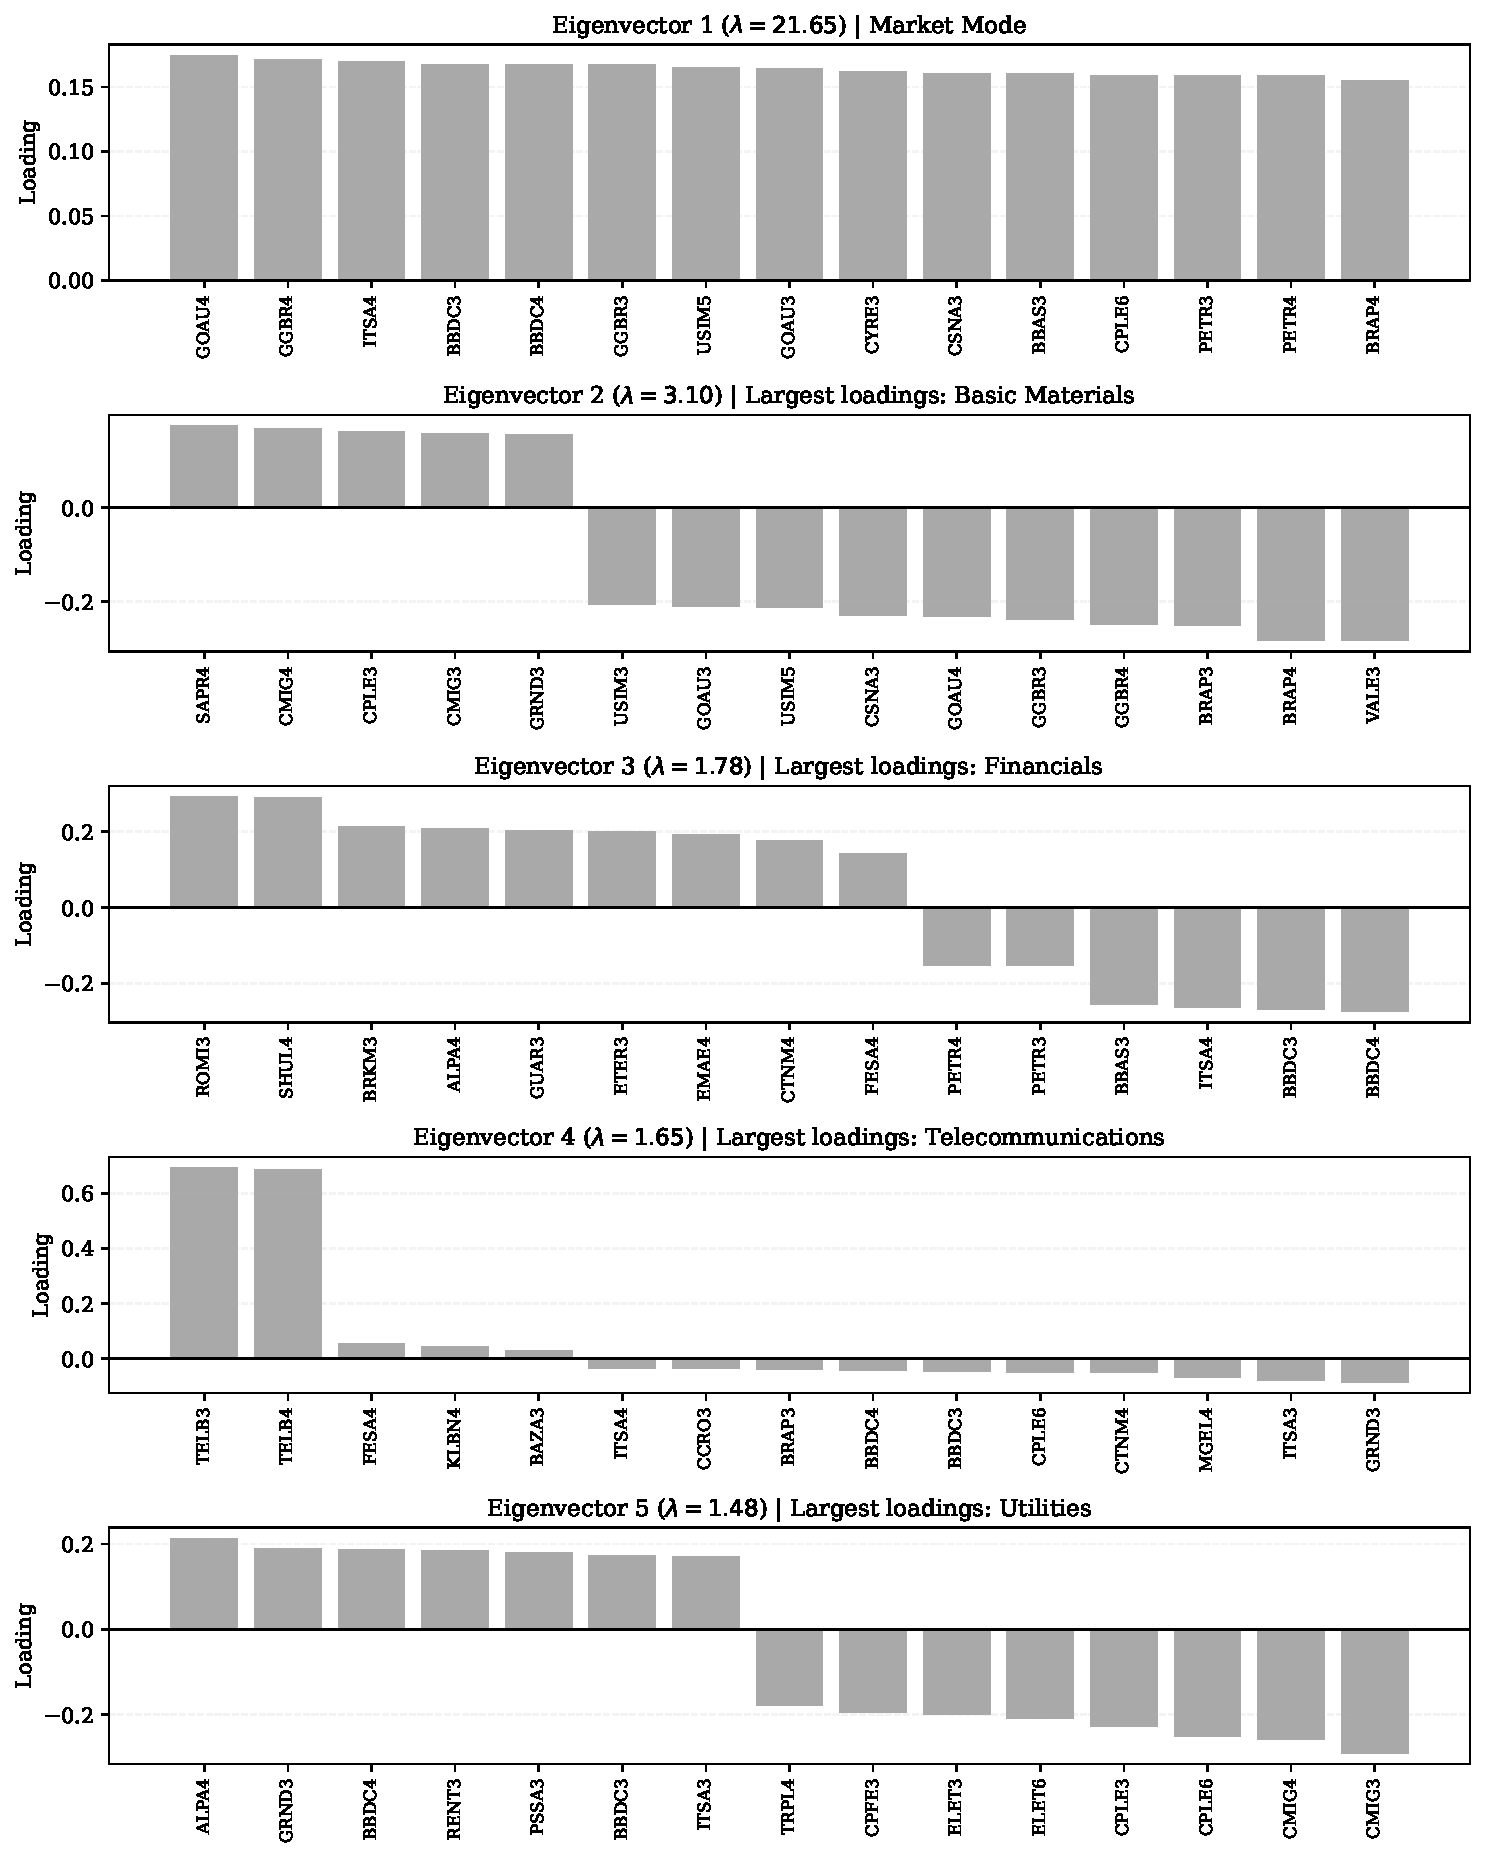
\includegraphics[width=\linewidth]{images/figure_7b_rmt_top_eigenvectors_top_loadings.pdf}
\captionof{figure}{Top eigenvector loadings for the leading RMT modes. Eigenvector 1 captures the market-mode component; subsequent eigenvectors are read as candidate group or localized sectoral components.}
\label{fig:eigenvector_loadings}
\end{center}


\subsection{Top eigenvector loadings}

Eigenvalues identify the strength of collective modes, but eigenvectors help interpret their composition. Figure~\ref{fig:eigenvector_loadings} reports the largest loadings for the leading eigenvectors. The first eigenvector captures the market-mode component because its loadings are broadly positive across the cross-section. We read subsequent eigenvectors as candidate group or localized components.

For each eigenvector, assets are ranked by the magnitude of their loadings. The signs of eigenvector loadings are arbitrary up to multiplication by $-1$, so interpretation focuses on relative grouping and magnitude, not sign alone.

The second eigenvector suggests a Basic Materials and commodity-related component. The third contains financial and cross-sector structure. The fourth and fifth eigenvectors are more localized, with Telecommunications and Utilities-like components appearing among the dominant loadings. These labels are economic readings of the loading patterns, not mechanical classifications. Eigenvectors can mix sectors when firms share macroeconomic, liquidity or balance-sheet exposures.
